\section{实验}
\label{sec:experiments}

实验按自下而上顺序报告：先分类器能力核查，再有效 GSD 与观测分配，再功效与基准，最后 oracle 阶梯与端到端现实检验。
不把定位提升写成导航贡献，也不把 \semSR 当作严格成功。
评价指标与可识别性判据见 \secref{sec:metrics}：若巡航档与原生档几乎不翻转，则预算分配策略不可识别。

\subsection{训练/验证曲线、类别加权与基线对标}
\label{sec:x1train}
审稿意见 C1 指出：本文此前从未报告损伤分类器在训练/验证集上的逐类表现，
因此``损伤头先失败''这一归因无法与``训练本身失败（数据/标签 bug）''区分。
我们据此补做三组对照实验，结果汇总于 \tabref{tab:cpv2} 与 \tabref{tab:traincurve}。

\paragraph{训练曲线：确有信号，但不跨事件泛化。}
按 \secref{sec:method} 的类别加权 + macro-F1 选择重训后，训练集 macro-F1 随 epoch 从 $0.22$ 单调升至 $0.49$--$0.57$
（\tabref{tab:traincurve}），说明分类器确实学到了区分损伤等级的视觉线索，排除``从未训练成功''这一竞争解释。
但验证集（hurricane-harvey、mexico-earthquake，与训练事件不相交）macro-F1 全程停留在 $0.21$--$0.25$，
不随训练集拟合程度提升而改善，验证损失反而缓慢上升（过拟合）。
这是一条干净的``训练内有信号、跨事件不泛化''曲线，构成事件级域偏移的直接证据，而不是训练流程 bug 的证据。

\paragraph{类别加权部分缓解塌缩，但未逆转。}
\tabref{tab:cpv2} 对比未加权（论文早期版本）与类别加权（当前版本）checkpoint：
测试集 macro-F1 从 $0.220$ 升至 $0.276$，``损毁''类召回从 $0.007$ 恢复到 $0.164$；
但``轻微损伤''与``严重损伤''召回仍接近 0。加权训练有效但不充分，核心瓶颈判断不变。

\paragraph{与标准（非事件不相交）切分对照，拆分协议难度与架构差距（C2）。}
本文刻意使用比公开 xBD 基线更严格的事件级切分（不同灾害事件，见 \secref{sec:x1train} 前言），
但由此产生的 macro-F1 $\approx 0.7$（文献常见数值）与本文 $\approx 0.28$ 之间的差距，
可能来自(i)评测协议更难，也可能来自(ii)本文架构/训练配方偏简单（轻量 ResNet18 双塔、8 epoch、无集成）。
我们用同一架构在\textbf{官方标准切分}（图像级随机切分，训练/测试可共享灾害事件，与文献协议一致）上重训一次以分离两个因素：
测试集 macro-F1 升至 $0.308$（\tabref{tab:cpv2} 末行）——比事件不相交高约 $0.03$--$0.04$，但仍远低于文献的 $\sim 0.7$。
据此，协议难度只能解释差距的一小部分（$\lesssim 0.04$），大部分差距（$0.31\to0.7$）应归因于架构/训练规模的局限，
应作为本文的诚实局限性陈述（\secref{sec:limitations}），而不是继续在本文内追赶公开基线的理由——
直接借用公开预训练权重会因其训练集覆盖本文全部 val/test/holdout 事件而构成泄漏（见 \secref{sec:related}、附录）。

\paragraph{H2：差分注意力与拼接融合无统计显著差异。}
\tabref{tab:cpv2} 第 2、3 行对比同一事件不相交切分下的两种融合方式：
拼接在验证集选择指标上略高（macro-F1 $0.241$ vs.\ $0.222$），差分注意力在测试集``损毁''召回上明显更高（$0.164$ vs.\ $0.055$），
两者互有胜负，样本量下不足以判定何者更优。H2 的结论是``在本数据规模下无法区分'', 而非任一方向的优势。

\begin{table}[htbp]
\centering
\caption{新旧 checkpoint、两种融合架构与两种切分协议的 macro-F1 / 逐类召回对照。}
\label{tab:cpv2}
\begin{tabular}{lrrrrrr}
\hline
checkpoint & train F1 & val F1 & test F1 & test 完好召回 & test 损毁召回 & 切分协议 \\
\hline
旧（未加权，论文原用） & 0.242 & 0.221 & 0.220 & 0.989 & 0.007 & 事件不相交 \\
v2 差分注意力（加权） & 0.348 & 0.222 & 0.276 & 0.973 & 0.164 & 事件不相交 \\
v2 拼接（加权，H2 对照） & 0.370 & 0.241 & 0.265 & 0.951 & 0.055 & 事件不相交 \\
标准切分拼接（加权，协议对照） & 0.330 & 0.350 & 0.308 & 0.995 & 0.233 & 标准（非事件不相交） \\
\hline
\end{tabular}

\end{table}

\begin{table}[htbp]
\centering
\caption{类别加权训练下的逐 epoch train/val macro-F1（C1 证据：训练内有信号、验证集不改善）。}
\label{tab:traincurve}
\begin{tabular}{llrrrr}
\hline
配置 & epoch & train macro-F1 & val macro-F1 & train acc & val acc \\
\hline
差分注意力（事件不相交，加权） & 1 & 0.220 & 0.222 & 0.735 & 0.797 \\
 & 2 & 0.275 & 0.208 & 0.735 & 0.673 \\
 & 3 & 0.336 & 0.224 & 0.757 & 0.755 \\
 & 4 & 0.376 & 0.224 & 0.787 & 0.754 \\
 & 5 & 0.400 & 0.216 & 0.796 & 0.720 \\
 & 6 & 0.414 & 0.215 & 0.798 & 0.719 \\
 & 7 & 0.438 & 0.220 & 0.804 & 0.745 \\
 & 8 & 0.486 & 0.223 & 0.804 & 0.786 \\
\hline
拼接（事件不相交，加权） & 1 & 0.242 & 0.232 & 0.729 & 0.788 \\
 & 2 & 0.294 & 0.219 & 0.733 & 0.704 \\
 & 3 & 0.325 & 0.213 & 0.737 & 0.683 \\
 & 4 & 0.411 & 0.247 & 0.784 & 0.783 \\
 & 5 & 0.449 & 0.208 & 0.807 & 0.675 \\
 & 6 & 0.498 & 0.225 & 0.814 & 0.782 \\
 & 7 & 0.541 & 0.220 & 0.819 & 0.774 \\
 & 8 & 0.568 & 0.224 & 0.824 & 0.779 \\
\hline
拼接（官方标准切分，加权） & 1 & 0.219 & 0.213 & 0.755 & 0.741 \\
 & 2 & 0.266 & 0.310 & 0.748 & 0.740 \\
 & 3 & 0.313 & 0.213 & 0.749 & 0.741 \\
 & 4 & 0.395 & 0.318 & 0.777 & 0.760 \\
 & 5 & 0.451 & 0.294 & 0.793 & 0.753 \\
 & 6 & 0.481 & 0.344 & 0.795 & 0.767 \\
 & 7 & 0.519 & 0.333 & 0.800 & 0.761 \\
 & 8 & 0.559 & 0.325 & 0.806 & 0.765 \\
\hline
\end{tabular}

\end{table}

\subsection{有效 GSD 与分类质量}
\label{sec:x1}
\tabref{tab:gsd} 给出重训后（类别加权、差分注意力）checkpoint 在巡航档到原生档的精度、macro-F1 与 ECE（$n=400$，事件不相交测试集）。
原生档预测为``完好''$381$、``损毁''$19$，巡航--原生预测翻转 $7$ 次（\tabref{tab:gsdcls}）。
配对 bootstrap 下原生档相对巡航档的精度差均值为 $-0.0025$，95\% 置信区间 $[-0.0125,\,0.0075]$ \textbf{含 0}，验收仍为 \texttt{accept\_native\_better=false}。
macro-F1 在五档间为 $0.273$--$0.286$，较未加权版本的 $0.184$ 平坦值有提升但仍以完好类为主。

为排除``$4\times$ 降质过弱''，另将尺度加到 $8\times$ 与 $16\times$（有效 GSD $4\,\mathrm{m}$ 与 $8\,\mathrm{m}$）：
预测分布与翻转次数无实质变化（单元测试确认降质本身会改变高频像素，因此不是空操作）。
当前损伤头对纹理的敏感度不足以支撑跨 GSD 的信息增益估计，但方向已不再反常——见图 \ref{fig:gsd}。

\begin{table}[htbp]
\centering
\caption{事件不相交测试裁块上的高度--GSD 阶梯（$n=400$，类别加权 checkpoint）。}
\label{tab:gsd}
\begin{tabular}{lrrrr}
\hline
尺度 / 有效 GSD & 精度 & macro-F1 & ECE & 平均熵 \\
\hline
1.00$\times$ / 0.50 m & 0.623 & 0.286 & 0.042 & 0.776 \\
1.75$\times$ / 0.88 m & 0.623 & 0.286 & 0.055 & 0.776 \\
2.50$\times$ / 1.25 m & 0.620 & 0.273 & 0.053 & 0.777 \\
3.25$\times$ / 1.62 m & 0.623 & 0.279 & 0.049 & 0.779 \\
4.00$\times$ / 2.00 m & 0.625 & 0.279 & 0.086 & 0.782 \\
\hline
\end{tabular}

\end{table}

\begin{table}[htbp]
\centering
\caption{同一测试裁块上的类别支持数、原生档预测数与召回。巡航--原生预测翻转 7 次。}
\label{tab:gsdcls}
\begin{tabular}{lrrr}
\hline
类别 & 标注数 & 原生档预测数 & 原生档召回 \\
\hline
完好 & 250 & 381 & 0.972 \\
轻微损伤 & 125 & 0 & 0.000 \\
严重损伤 & 12 & 0 & 0.000 \\
损毁 & 13 & 19 & 0.462 \\
\hline
巡航$\leftrightarrow$原生预测翻转 & \multicolumn{3}{r}{7} \\
\hline
\end{tabular}

\end{table}

\begin{figure}[htbp]
\centering
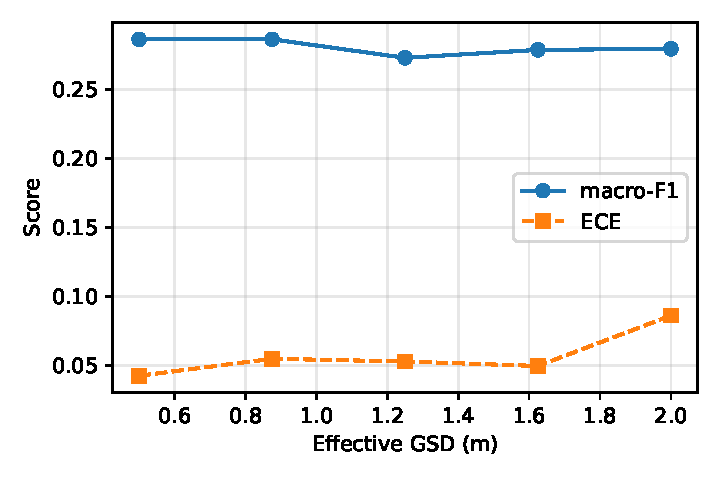
\includegraphics[width=0.72\linewidth]{generated/gsd_ladder.pdf}
\caption{有效 GSD 与 macro-F1 / ECE。macro-F1 大致平坦；平均熵随 GSD 变粗\textbf{单调上升}——
方向与``下降应降低不确定性''的假设一致（未加权版本曾观察到方向相反，见附录变更记录），
但幅度很小，仍不足以支撑稳健的跨 GSD 触发决策。}
\label{fig:gsd}
\end{figure}

\subsection{预算受限观测分配}
\label{sec:x2}
设定：每样本平均允许 $B\in\{0,0.1,0.25,0.5,1.0\}$ 次原生档观测。
策略为不下降、随机、未校准熵、校准熵、条件期望熵、共形集合以及已知标签是否翻转的 oracle。
类别加权 checkpoint 重跑后，400 个配对样本中巡航预测与原生预测相差 $7$ 例（$n_{\mathrm{flip}}=7$，较未加权版本的 $1$ 例增加，
但绝对量仍很小）。\tabref{tab:budget} 中各策略在 $B=0.25$ 时 macro-F1 集中在 $0.277$--$0.286$，
oracle 参照与不下降之间的差距仅 $0.0094$，\texttt{accept\_calibrated\_better=false} 依旧成立。
可分配信息量随分类器改善而略有增加（$n_{\mathrm{flip}}$ 从 1 到 7），但幅度仍不足以让任何触发策略在宏观 F1 上跑赢随机或不下降。
表中 ECE 出现约两倍分离（不下降 $0.086$，未校准/校准熵约 $0.038$）：这与温度缩放不改变 $\arg\max$ 相符，说明机制作用在概率而非标签；宏观 F1 平坦不能单独写成``校准无用''。
这与 \secref{sec:x1train} 的判断一致：分类器改善方向正确，但当前规模不足以让下降--居中动作产生可辨识的\textbf{定类}收益。

\begin{table}[htbp]
\centering
\caption{平均每样本额外观测 $B=0.25$ 时的损伤判定（$n=400$，类别加权 checkpoint，$n_{\mathrm{flip}}=7$）。}
\label{tab:budget}
\begin{tabular}{lrrr}
\hline
策略 & macro-F1 & 精度 & ECE \\
\hline
不下降 & 0.279 & 0.625 & 0.086 \\
随机 & 0.286 & 0.623 & 0.074 \\
未校准熵 & 0.286 & 0.623 & 0.037 \\
校准熵 & 0.286 & 0.623 & 0.038 \\
条件期望熵 & 0.277 & 0.625 & 0.050 \\
Conformal & 0.286 & 0.627 & 0.071 \\
Oracle 参照（非上界） & 0.286 & 0.623 & 0.078 \\
\hline
\end{tabular}

\end{table}

\begin{figure}[htbp]
\centering
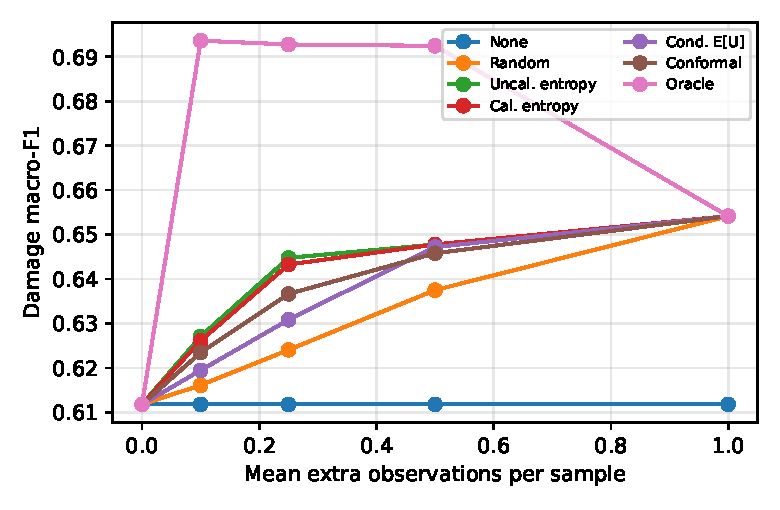
\includegraphics[width=0.78\linewidth]{generated/budget_allocation.pdf}
\caption{额外观测预算与损伤宏观 F1。各策略曲线高度重叠；oracle 曲线是逐样本翻转参照而非宏观 F1 上界。}
\label{fig:budget}
\end{figure}

超参 $\tau\in\{0.3,0.4,0.5,0.6,0.7\}$ 只改变下降次数，macro-F1 基本不变，敏感性分析在当前分类器规模下仍缺乏信息量。

\subsection{功效分析与事件隔离基准}
\label{sec:x4x5}
旧设计 40 题 $\times$ 3 种子、6 策略 Holm 校正下，最小可检测严格 SR 约为 9.6 个百分点（基线 SR$=0.05$、功效 $0.8$），远大于 plausible 的 2--5 个百分点效应，故``本次不显著''在设计上接近``永不显著''。
功效 0.8 检测 5 个百分点增益约需每策略 444 题。
新基准为 200 题，仍欠功效约 $2.2$ 倍，故后文端到端各策略 \SR 同质应读作\textbf{欠功效下的非结果}，而不是已经证伪了 2--5 个百分点的效应。
新 evidence-rich 草稿仅含 test+holdout 事件（hurricane-michael、palu-tsunami、moore-tornado、nepal-flooding、pinery-bushfire），200 题中 easy/medium/hard 为 75/70/55，含 33 条多地标；审核字段为``模型辅助审核 + 作者抽查''，生成脚本对 train/val 事件断言失败。
在损伤头召回未恢复前，扩大题库不能单独挽救 X2。

\begin{table}[htbp]
\centering
\caption{六策略 Holm 校正下的样本量规划。表中 0.0962 是相对基线 \SR 的最小可检测差值，不是成功率本身。}
\label{tab:power}
\begin{tabular}{lr}
\hline
量 & 取值 \\
\hline
基线 SR & 0.05 \\
目标绝对增益 & 0.05 \\
Holm $\alpha$ & 0.01 \\
功效 0.8 所需每策略题数 & 444 \\
旧设计最小可检测 SR & 0.0962 \\
\hline
\end{tabular}

\end{table}

\subsection{RescueNet 低空评估域}
\label{sec:rescuenet}
RescueNet 为 Hurricane Michael 无人机影像，建筑损伤按 FEMA 四级标注，与 xBD 四类直接映射\cite{rahnemoonfar2023rescuenet}；数据来自 Scientific Data/figshare 的 CC BY 4.0 发布，仅评估、不训练。
该数据集无灾前配对，双时相输入将灾后裁块复制为灾前通道（差通道\textbf{恒为} 0，不是近似为 0）。
这一输入构造本身就保证``无变化$\to$完好''是数学必然，而不是域漂移的独立证据：
本节结果因此\textbf{只}度量卫星训练分类器在真实低空外观上的漂移，不能作为``绑定约束在损伤头而非卫星 GSD''的独立支持证据；
后者需要单时相（仅灾后）分类头对照，本文暂未实现，留作后续工作。
FloodNet 因只有淹没/未淹没二值标签且与四级损伤不对齐，不引入。
类别加权 checkpoint 重跑结果与塌缩模式一致：完好类召回为 $1.00$，三类损伤召回均为 0；
精度 $0.210$、macro-F1 $0.087$、ECE $0.421$（\tabref{tab:rescue}）。

\begin{table}[htbp]
\centering
\caption{卫星训练分类器在 RescueNet 测试影像上的零样本漂移（灾后裁块复制为灾前）。}
\label{tab:rescue}
\begin{tabular}{lrr}
\hline
项 & 支持数 & 指标 \\
\hline
图像数 & 80 & -- \\
建筑连通域 & 181 & -- \\
精度 & -- & 0.210 \\
macro-F1 & -- & 0.087 \\
ECE & -- & 0.421 \\
\hline
完好召回 & 38 & 1.000 \\
轻微损伤召回 & 41 & 0.000 \\
严重损伤召回 & 22 & 0.000 \\
损毁召回 & 80 & 0.000 \\
\hline
\end{tabular}

\end{table}

\subsection{端到端缺陷与探索回退}
\label{sec:x0x3}
对历史全零结果的排查结论如下。
\begin{enumerate}
\item 旧题库首题起点--目标距离 $48.19\,\mathrm{m}$，北向 $-20.8\,\mathrm{m}$、东向 $43.5\,\mathrm{m}$，不符合 lat/lon 互换的几何签名。
\item E1 与 E11 使用同一 evidence-rich 题库；在复检从未触发时，B1--B3 与六策略轨迹级聚合相同是预期现象，不是串台。
\item LLM/VLM 不可达时，分层规划对无方向先验题每步默认向北，$12\times 90\,\mathrm{m}$ 量级位移与平均 NE $587.6\,\mathrm{m}$ 相符。已改为螺旋搜索，单测验证连续四步不再恒为北。
\item \textbf{零提议根因（第二处独立缺陷）}：U-Net 定位器推理时把任意输入 resize 到训练尺寸，$256\,\mathrm{px}$ 机载视场被上采样后建筑尺度偏离训练分布，提议塌缩为 0——同一权重在完整 $1024\,\mathrm{px}$ 瓦片上产生 95 个提议，在 256 视场上为 0。
修复为：对灾前底图整瓦片做一次原生分辨率定位（进程内缓存），再把落进当前视场的框平移到视场坐标；且灾前底图是离线卫星产品，其分辨率与无人机当前高度无关，不再随 GSD 阶梯降质，只有灾后实时观测降质。
修复后单题 trace 每步产生 2--10 个建筑提议、损伤分类器全部被调用（此前全程为 0），证据链路首次完整执行。
\item 修复后损伤证据以``完好''为主：分类器对少数``损毁''案例已有一定命中（\secref{sec:x1train}），但``轻微/严重损伤''证据仍几乎不出现，与 \secref{sec:x1} 的离线结论闭环——瓶颈不在导航或定位，在损伤头对中间损伤等级的召回。
\item \textbf{VLM 恢复与混合指认验证}：视觉语言模型改为进程内 Transformers 直接加载 Qwen2.5-VL-7B（本地权重、离线可复现，不依赖外部推理服务），混合指认路径（检测器优先、VLM 兜底）真实生效。
\item \textbf{早停缺陷（第三处独立缺陷）}：两个规划器在目标进入判到达半径（$35\,\mathrm{m}$）后原地停止而不平移到目标上方，而成功半径为 $25\,\mathrm{m}$，构成系统性早停。修复为判到达后先对准目标再停止。
\item 修复后单题 trace 暴露新的真实误差源：VLM 在起点视场内指认了一处``完全损毁建筑''（视场内 $19\,\mathrm{m}$），但对齐 GT 足迹后该位置 $61\,\mathrm{m}$ 内无损毁建筑，属开放词汇指认误报。这类误报不是实现缺陷，而是需要复检机制去纠偏的对象——但复检又受损伤头塌缩约束，两个失效源在端到端层面耦合。
\end{enumerate}

\subsection{Oracle 阶梯与端到端现实检验}
\label{sec:x3x6}
在全部修复后的栈上，于事件隔离基准（200 题）重跑：(i) oracle 阶梯 L0--L3（\tabref{tab:oracle}），交叉解耦导航与指认；(ii) 主消融 B0--B3 与复检策略族、GPS 定位扰动（$\sigma\in\{2,5,10\}\,\mathrm{m}$）及强制退化几何套件（\tabref{tab:e2e}）。
解释时须注意：在损伤头塌缩的前提下，任何配置的损伤证据与复检触发都受同一上游约束。

\paragraph{L2 是 oracle 初始定位，不是 oracle 导航。}
L2 的实现是回合开始即把无人机放到目标正上方，指认模块此后仍照常运行、仍可将其重新拉离目标——
导航/运动闭环本身从未被替换或屏蔽。因此 L1$-$L2 的差值度量的是``指认 vs.\ 初始位置''，不是``指认 vs.\ 导航''，
下文改称 L2 为``oracle 初始定位''，避免层间归因被误读为对导航模块的检验。真正的 oracle 导航（屏蔽指认对运动的影响）留作后续工作。

\paragraph{瓶颈定位在指认层。}
oracle 阶梯给出层间归因：仅替换指认（L1）即把严格 SR 从 $0.08$ 提升到 $1.00$（NE $0.1\,\mathrm{m}$、SPL $0.986$），说明指认正确时规划--运动闭环几乎无损；
而仅替换初始定位（L2）——不屏蔽指认——SR 只有 $0.50$：一半的题在到达后仍被开放词汇误指认重新拉离目标。
两者对比表明目标指认是当前剩余瓶颈的主要来源：检测器路径受限于损伤头对中间损伤等级的低召回，VLM 路径则存在 \secref{sec:x0x3} 所示的开放词汇误报，二者叠加构成 L0 的低 SR。
这一结论的边界条件须明确：仿真不含风扰、避障与能耗约束，$\mathrm{SR}=1.00$ 说明``指认正确时该仿真的运动学假设下闭环无损''，
不能外推为``导航与运动闭环对真实飞行不再是短板''。

\paragraph{端到端上机制不可辨识，与离线分水岭闭环。}
主消融 B0--B2 的 SR 在 $0.07$--$0.08$ 之间同质，记忆拓扑图（B3）反而使 NE 变差（$305.7\,\mathrm{m}$）。
五种复检策略（随机、固定、校准熵、条件期望熵、conformal）SR 完全相同（$0.08$），200 题中触发 0--3 次：
损伤证据几乎不存在时，任何触发准则都退化为``从不触发''。
这与 \secref{sec:x2} 的离线结论在端到端层面闭环——不是复核机制失败，而是它从未获得可复核的输入。

\paragraph{几何扰动不是当前瓶颈；强制退化几何下 SR 显著更低，但样本量不足以单独立因果论证。}
GPS 起点扰动 $\sigma$ 从 0 增至 $10\,\mathrm{m}$，SR 在 $0.065$--$0.095$ 间非单调波动，量级远小于指认噪声，几何鲁棒性尚未成为可观测约束。
强制退化几何（禁用检测框地理投影与复检居中）使 SR 降至 $0.025$、全部回合耗尽 12 步预算、NE 升至 $414\,\mathrm{m}$，
Fisher 精确检验显示该组（$k=\DegradedFisherDegK{}/n=\DegradedFisherDegN{}$）与主套件 B2（$k=\DegradedFisherBaseK{}/n=\DegradedFisherBaseN{}$）SR 差异 $p=\DegradedFisherP{}$
（\tabref{tab:e2e} 给出各组 95\% Wilson 置信区间）。
我们只报告该条件下的观测 SR 与显著性检验结果，不把``禁用投影''单一处理下的差异直接推广为``投影通道是到达能力的必要成分''这一更强的因果断言——
消融同时改变了投影与复检居中两个环节，无法互相分离。

\begin{table}[htbp]
\centering
\caption{Oracle 阶梯：导航与指认逐层替换为 oracle 后的到达能力（事件隔离基准，$n=200$）。}
\label{tab:oracle}
\begin{tabular}{llrrrrr}
\hline
层级 & 设定 & $n$ & SR (95\% CI) & semSR & NE (m) & SPL \\
\hline
L0 & 无 oracle（现状） & 200 & 0.080 [0.050,0.126] & 0.155 & 223.9 & 0.068 \\
L1 & oracle 指认 & 200 & 1.000 [0.981,1.000] & 1.000 & 0.1 & 0.986 \\
L2 & oracle 初始定位（指认仍生效） & 200 & 0.500 [0.431,0.569] & 0.550 & 148.5 & 0.381 \\
L3 & oracle 初始定位+指认 & 200 & 1.000 [0.981,1.000] & 1.000 & 0.0 & 1.000 \\
\hline
\end{tabular}

\end{table}

\begin{table}[htbp]
\centering
\caption{端到端主消融与扰动套件（事件隔离基准）。\SR 附 Wilson 95\% 置信区间。
固定下降策略触发次数远小于回合数，因为触发仍受上游``存在损伤证据''门控。}
\label{tab:e2e}
\begin{tabular}{llrrrrr}
\hline
套件 & 配置 & $n$ & SR (95\% CI) & semSR & NE (m) & 复检触发 \\
\hline
主套件 & B0 & 200 & 0.070 [0.042,0.114] & 0.165 & 222.3 & 0 \\
主套件 & B1 & 200 & 0.080 [0.050,0.126] & 0.155 & 223.9 & 0 \\
主套件 & B2 & 200 & 0.080 [0.050,0.126] & 0.155 & 223.9 & 0 \\
主套件 & B3 & 200 & 0.080 [0.050,0.126] & 0.140 & 305.7 & 0 \\
复检策略族 & E11\_RANDOM & 200 & 0.080 [0.050,0.126] & 0.155 & 223.9 & 0 \\
复检策略族 & E11\_FIXED & 200 & 0.080 [0.050,0.126] & 0.155 & 224.0 & 3 \\
复检策略族 & E11\_ENTROPY & 200 & 0.080 [0.050,0.126] & 0.155 & 223.9 & 1 \\
复检策略族 & E11\_INFOGAIN & 200 & 0.080 [0.050,0.126] & 0.155 & 223.9 & 2 \\
复检策略族 & E11\_CONFORMAL & 200 & 0.080 [0.050,0.126] & 0.155 & 223.9 & 2 \\
GPS $\sigma{=}2$ m & B2 & 200 & 0.065 [0.038,0.108] & 0.140 & 230.7 & 1 \\
GPS $\sigma{=}5$ m & B2 & 200 & 0.085 [0.054,0.132] & 0.155 & 221.4 & 0 \\
GPS $\sigma{=}10$ m & B2 & 200 & 0.095 [0.062,0.144] & 0.200 & 238.6 & 0 \\
强制退化几何 & B2 & 200 & 0.025 [0.011,0.057] & 0.075 & 414.4 & 0 \\
\hline
\end{tabular}

\end{table}
